%! Author = tstreule

\section{MRI}

\subsection{Quantum basics}
\textbf{Spin} $S_z = \hbar m \quad m = -I, -I+1, ... I \quad |S| = \hbar \sqrt{I(I+1)}$\\
\textbf{Magnetic moment}: \fbox{$\vec{\mu} = \gamma \vec{S}$} ($\gamma$: gyromagnetic ratio)\\
\textbf{Energy content} in $\vec{B}$-Filed: \fbox{$E_m = -\vec{\mu} \cdot \vec{B} = \pm \frac{\hbar}{2} \gamma B_0$}\\
\textbf{Blotzmann stat.}: $\frac{n\ped{-1/2}}{n\ped{+1/2}} = \exp(-\frac{\Delta E_m}{k\ped{B} T})$ \quad $\frac{\Delta n}{n} \propto \frac{\gamma \hbar B_0}{2 k\ped{B} T}$\\
\textbf{Larmor frequency}: E gap $\leftrightarrow$ photons: \highlight{$\displaystyle \omega_L = \gamma B_0$}\\
\textbf{Macrosc. mag. dipolar moment}: \fbox{$\vec{M}_0 = \sum \vec{\mu} = \Delta n \mu_z$}

\textbf{Bloch equation} ($T_2 << T_1$)\\
\highlight{$\displaystyle \frac{d}{dt}\vec{M} = \left( \begin{matrix}
                                        -1/T_2 & -\gamma B_z & \gamma B_y \\
                                        \gamma B_z & -1/T_2 & -\gamma B_x \\
                                        -\gamma B_y & \gamma B_x & -1/T_1\end{matrix} \right) \vec{M} + \left( \begin{matrix}
                                                                                                                   0 \\ 0 \\ M_0 / T_1 \end{matrix} \right)$}\\
{\small $M_z(t) = M_0\cos\alpha + (M_0-M_0\cos\alpha) (1-\exp(-t/T_1))$, \hfill $\alpha = \gamma B_1\tau\ped{B1}$: tip angle}

$\vec{B}$ with $|\vec{B}| = B_1 = const$ and $B_z = B_0$ spinning with $\omega_{RF}$ around the z-Axis. $\omega_{RF} = \omega_L \iff \vec{M}$ spins $\downarrow, \uparrow, \downarrow$ etc.

\textbf{Rot. frame of reference}: $\vec{B}$ stays at a slight angle and $\vec{M}$ rotates around it. Correction: $B_z = B_0 - \omega_{RF} / \gamma$
%%%%%%%%%%%%%%%%%%%%%%%%%%%%%%%%%%%%%%%%%%%%%%%%%%%%%%
\subsection{Basic setup}
\begin{minipage}{\linewidth}
    \begin{enumerate}
        \item Have $B_z$ + rot. field to push spins in x-y-plane.
        \item Coils to make gradients: Maxwell (z), and two Golay pairs
        \item Changing the gradient $\to$ travel k-space and sample it
        \item IFFT to get the image weighted with proton density
    \end{enumerate}
\end{minipage}

Signal from entire obj: \qquad $S(t) = \eu^{\iu \omega_0 t} \int\ped{obj} \rho(\vec{r})\eu^{\iu \vec{k} (t) \cdot \vec{r}} \diff^3 \vec{r}$\\
Fourier transform of $\rho(\vec{r})$: \quad $S(\vec{k}) = \eu^{-\iu \omega_0 t} \int\ped{obj} \rho(\vec{r})\eu^{-\iu \vec{k} \cdot \vec{r}} \diff^3 \vec{r}$

\textbf{Slice sel.}: Grad. in z-dir. and flip spins with a sinc$\times$gauss-pulse ($\approx \laplace$ rect, range of freq. where $\Delta B_z = 0$).

Grad. $\to$ \textbf{dephasing}. $\implies$ invert G to \textbf{rephase} spins.

\subsubsection{Measuring the spin}
\fbox{$\hat{U}\ped{ind} = \iu\omega I_0^{-1} \hat{\vec{\mu}} \cdot \hat{\vec{B}}^t(\vec{r}) = M_{xy} V s(\vec{r})$}\\
\highlight{$\displaystyle s(\vec{r}) = \iu\omega I_0^{-1} (\hat{B}^t_x(\vec{r}) - \iu\hat{B}^t_y(\vec{r}))$} \highlight{$\displaystyle B_1^{(-)} = s/(\iu\omega)$}\\
$I_0$: Transmit current, $B^t$: Field received at $\vec{r}$ when transmitting, $s$: \textbf{Coil sensitivity}, $\hat{\vec{\mu}} = V(M_{xy}, -\iu M_{xy}, 0)^T$,

s of smaller coil $\uparrow$. \quad Large distance: s of bigger coil $\uparrow$

Signal $\propto \frac{dM}{dt} = \iu\omega_0 M_0 \eu^{\iu\omega_0 t} \highlight{\propto \gamma^3}$
%%%%%%%%%%%%%%%%%%%%%%%%%%%%%%%%%%%%%%%%%%%%%%%%%%%%%%
\subsection{Measurement procedures (All Gradient Echo)}
\textbf{Echo-planar imaging (EPI)}: 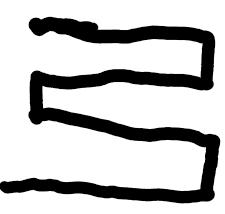
\includegraphics[width = 0.03\linewidth]{MRI_EPI}, spiral, radial

\begin{minipage}{.7\linewidth}
    $\circlearrowright \theta$, $T_E$, sample, $T_R-T_E$, again\\
    $\highlight{I \propto \rho \frac{(1-\eu^{-T_R/T_1})\sin \theta}{1 - \eu^{-T_R/T_1}\cos\theta} \eu^{-T_E/T_2}}$\\
    $\alpha\ped{Ernst} = \arccos (\eu^{-T_R/T_1})$

    \textbf{Sat. method}: \fbox{$1-\exp(-t/T_1)$} $T_E \approx 0$, $T_R \downarrow$ $\implies$ $T_1$ weighted. \textbf{Inv. recovery} also $T_1$\\
\end{minipage}%
\begin{minipage}{0.3\linewidth}
    \raggedleft
    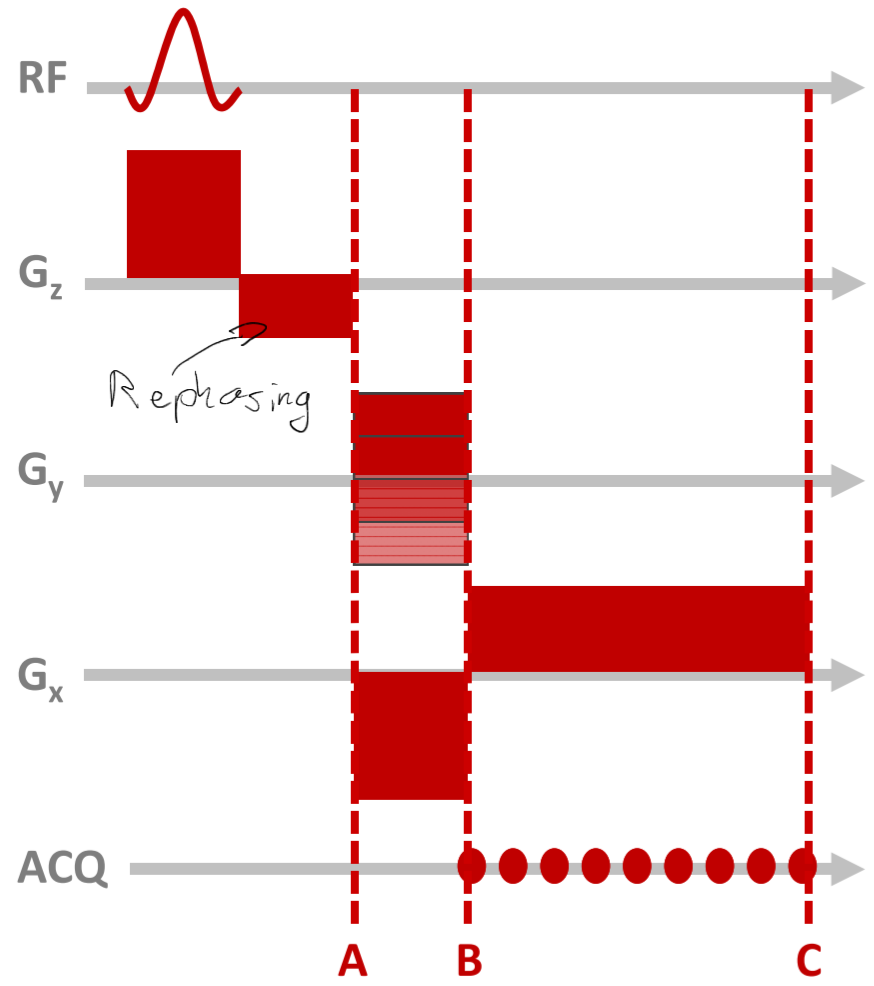
\includegraphics[width = .9\linewidth]{MRI_GradientEcho}
\end{minipage}\\
\textbf{Spin-echo method}: \fbox{$\exp(-t/T_2)$} $T_2^*$ decay (\textbf{const. loc. inhomog.}). $\circlearrowright$ at $T_E/2$ by 180°. $T_E \uparrow$ $\implies$ $T_2$ weight.

Saturation Method \quad $|$ Spin Echo Method\\
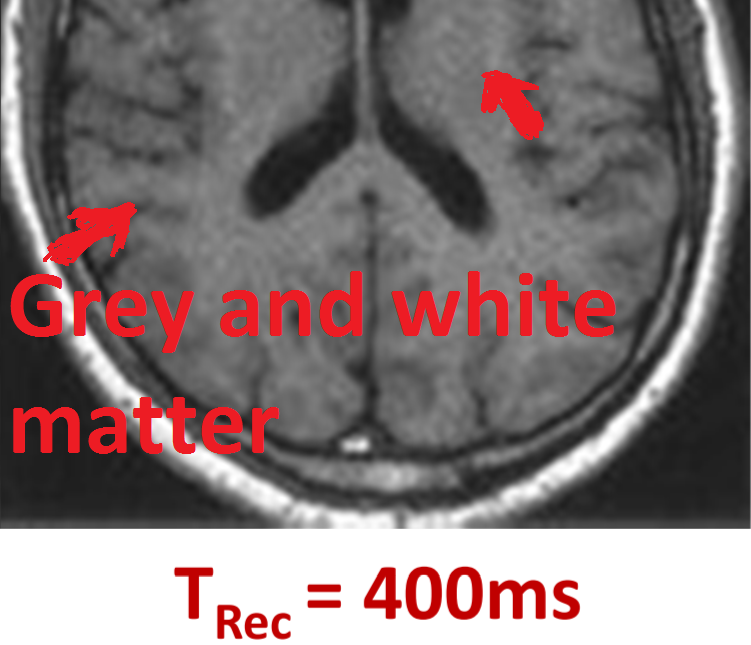
\includegraphics[width = 0.2\linewidth]{MRI_SatMethodShort}
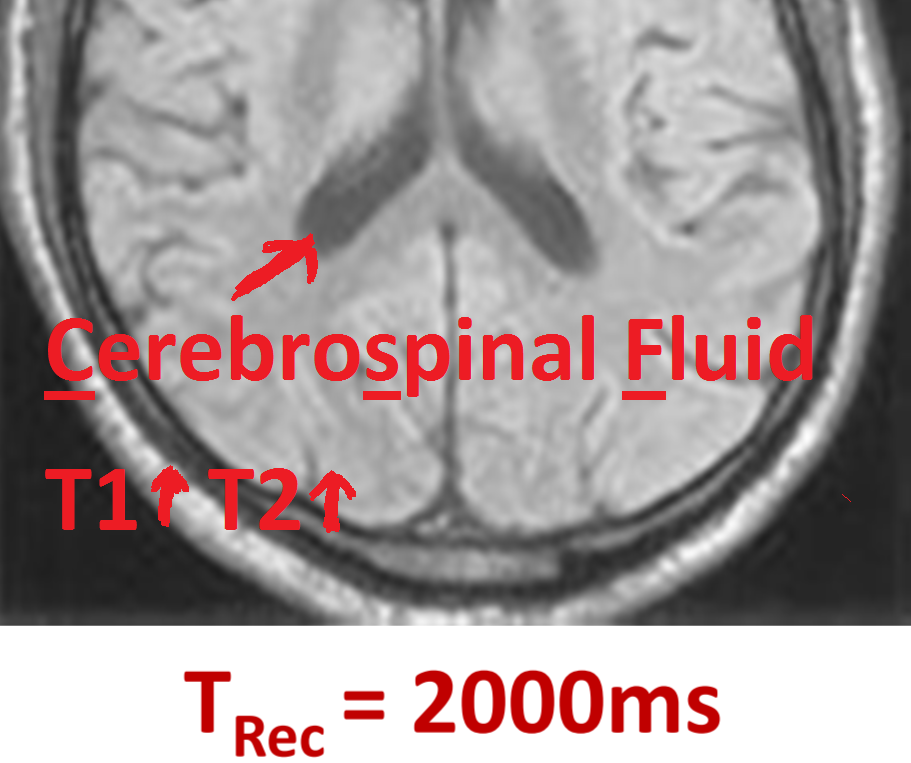
\includegraphics[width = 0.2\linewidth]{MRI_SatMethodLong}
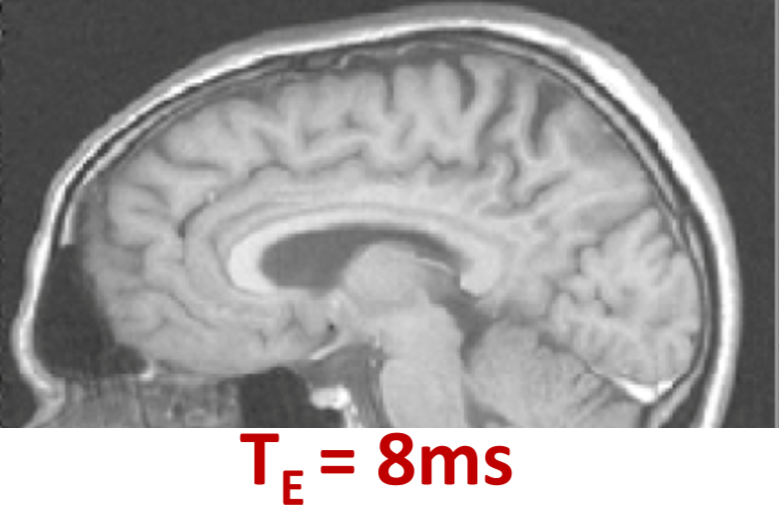
\includegraphics[width = 0.25\linewidth]{MRI_SpinEchoShort}
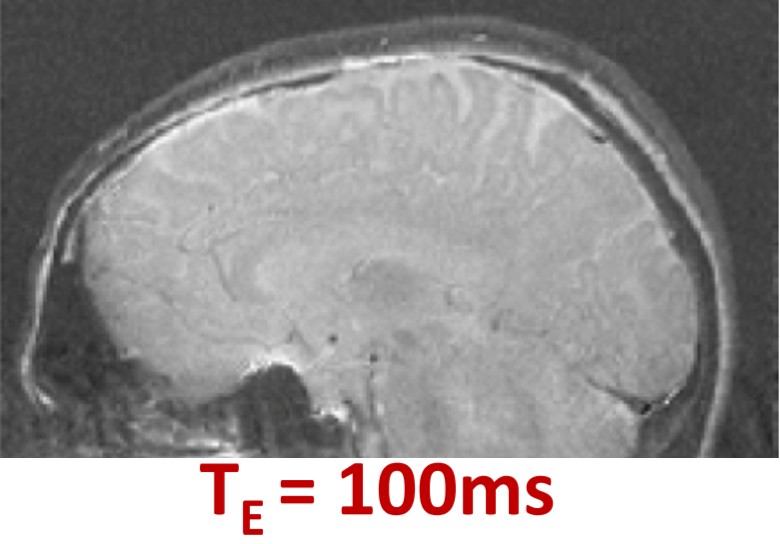
\includegraphics[width = 0.24\linewidth]{MRI_SpinEchoLong}

\textbf{Inflow contrast}: $T_1$ weight. (Blood with $\uparrow M_z$ during $T_R$)
%%%%%%%%%%%%%%%%%%%%%%%%%%%%%%%%%%%%%%%%%%%%%%%%%%%%%%
\subsection{Noise, SNR and Resolution}
$\sigma^2\ped{noise} = 4 k_B \cdot T \cdot R \cdot BW$ \hfill $T$: Temp., $R=U/I$, $BW$: Bandwidth

If frequency indep. and uniform $T$ ($I_0$ is transmit c.):\\
$\highlight{\sigma^2_{noise} = 4 k_B \cdot T \cdot BW \int \sigma(\vec{r}) \frac{\abs{\vec{E}(\vec{r})}^2}{I_0^2}dV}$

Otherwise: $\sigma^2\ped{noise} = 4 k_B \iint T(\vec{r}) \sigma(\omega, \vec{r}) \frac{\abs{\vec{E}(\omega, \vec{r})}^2}{I_0^2} \frac{d\omega}{2\pi} dV$

\fbox{$\sigma^2\ped{noise} = 4 k\ped{B} \cdot BW (R\ap{eff}\ped{sample} T\ped{sample} + R\ap{eff}\ped{coil} T\ped{coil} + R\ap{eff}\ped{env} T\ped{env})$} (last Term usually negligable)

\fbox{$\textbf{SNR} = \frac{\omega B_1^{(-)} (\vec{r}) M_{xy}(\vec{r}) \Delta V}{\sqrt{4 k_B BW (T_{sample}R_{sample} + T_{coil}R_{coil})}} \sqrt{N_{avg}}$}

$BW \propto \text{Gradient strength} \quad \propto \text{Body size} \quad \propto t\ped{acq}^{-1}$\\
$\quad t_{scan} \propto N_{avg} \quad \implies \highlight{SNR \propto \Delta V \sqrt{t}}$

SNR$\uparrow$: magnetization$\uparrow$ by $B_0\uparrow$. $\omega\uparrow$. $T\ped{coil}\downarrow$, $R\ped{coil}\downarrow$

\textbf{Resolution limits}:\\
In k-space, the image is multiplied with\\
$H(k) = \textrm{rect}\left( \frac{k}{2 k\ped{max}}\right) \eu^{-t/T_2^*} \quad \implies \textbf{PSF}:\: \highlight{\Delta x \geq \frac{\pi}{\gamma G\ped{max} T_2^*}}$\\

Diffusion Area: $\left< \Delta x^2 \right> = 6 \cdot D \cdot T\ped{acq}$ \hfill $D = \unitfrac[10^{-3}]{mm^2}{s}$ for $\ce{H_2O}$.
%%%%%%%%%%%%%%%%%%%%%%%%%%%%%%%%%%%%%%%%%%%%%%%%%%%%%%
\subsection{Various}
\textbf{T/R Switch}: Block kW in transmit mode, nW in r mode.

\textbf{RF Body Coil - Gradients - $B_0$-Magnet (3-7T) - Shield Coils - Cryogenics} @4K.

\fbox{$\unit[1]{Gauss} = \unit[0.1]{mT}$} \textbf{Limits}: 5 Gauss: Pacemakers, Credit cards. --- 50 Gauss magnetic objects

\subsubsection{fMRI \textnormal{-- functional MRI (brain imaging)}}
Oxygenated hemoglobin is diamagnetic, deoxy-Hb is paramagnetic. Param. disturbs the B-field $\implies$ reduces $T_2^*$. $S_{task} > S_{idle}$. Use echo planar imaging because it is fast.\\
Calc \textbf{scalar product} of activation and \textbf{paradigm} ($\pm 1$)
